\section{Organizacja} 
\begin{figure}[H]
\centering
 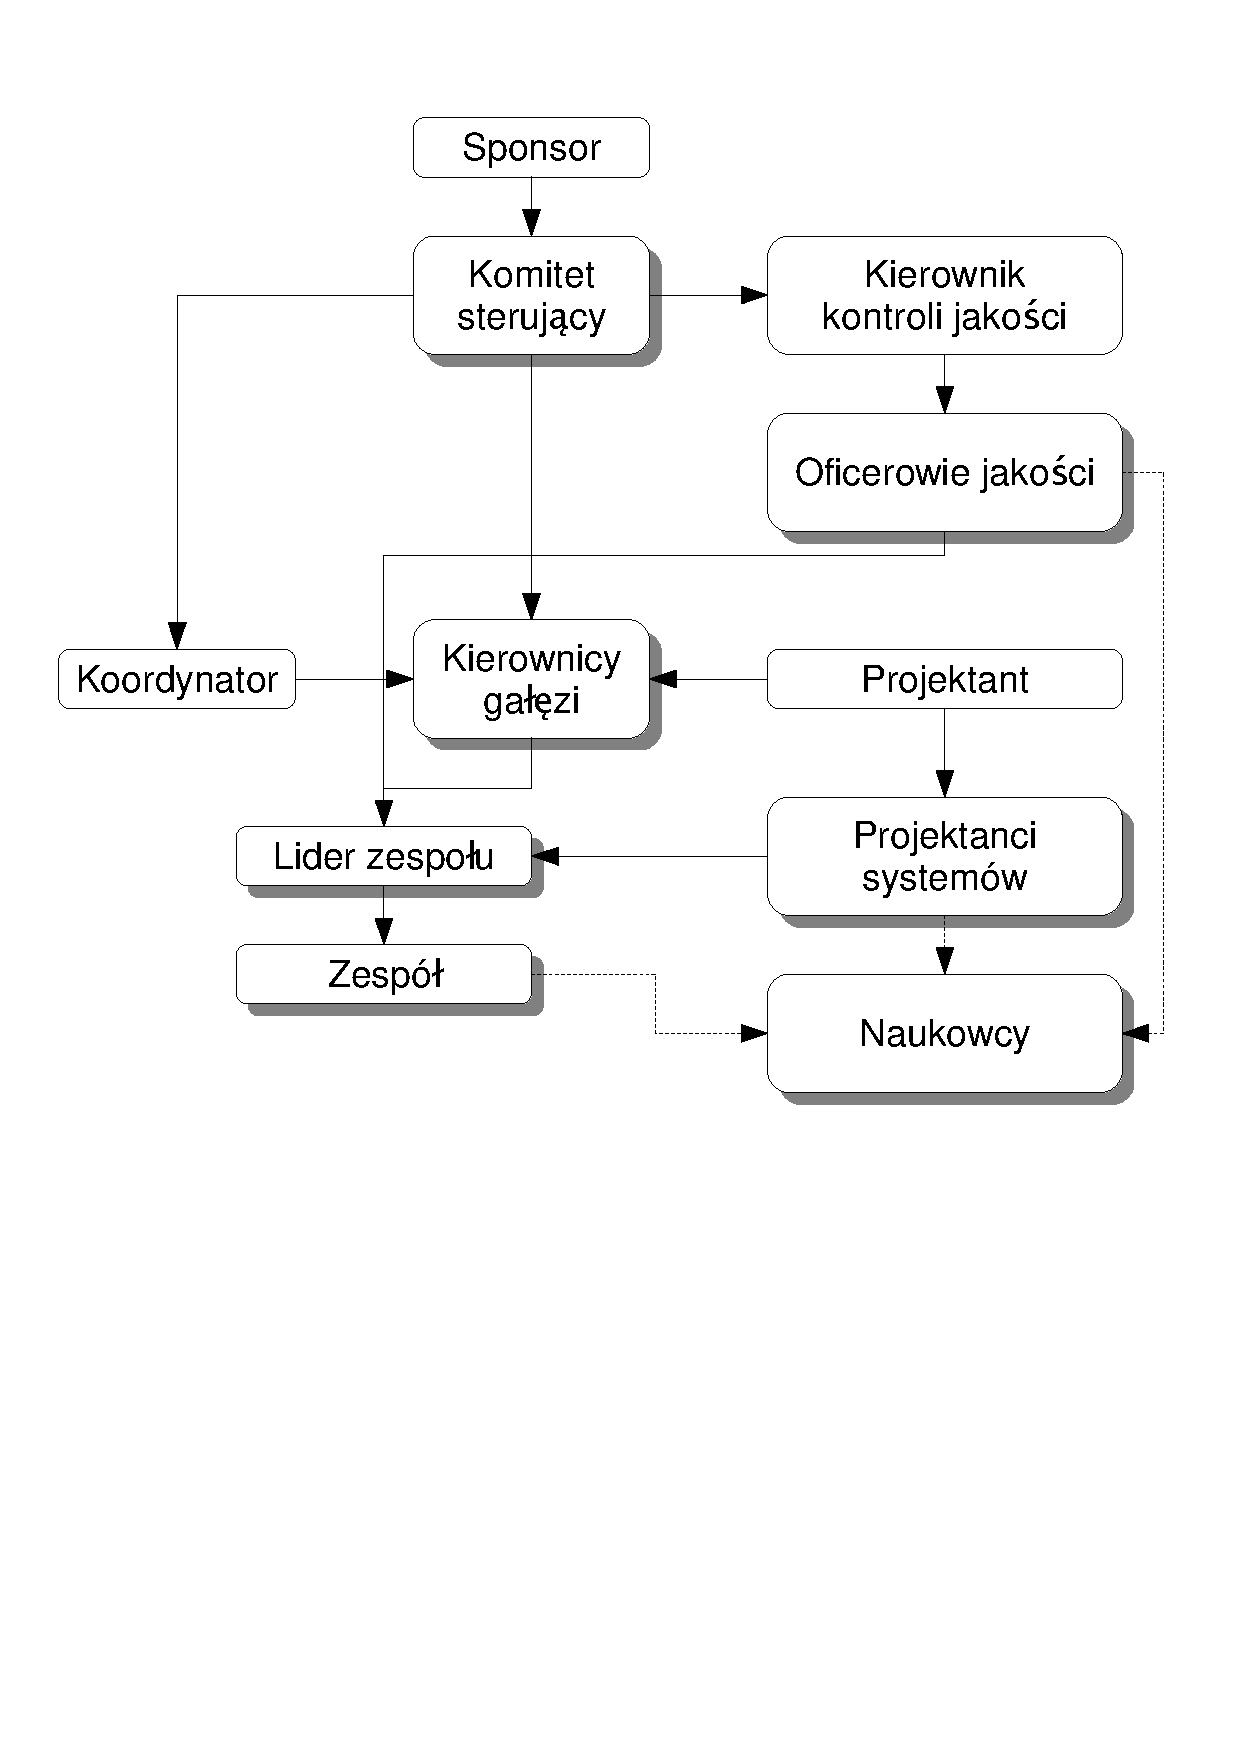
\includegraphics[width=\textwidth]{img/struktura.pdf}
\caption{Zarys zależności stanowisk projektu.}
\end{figure}
\subsection{Sponsor}
Sponsorem będzie sam prezydent Islandii.
Będzie on zarządzał finansowaniem projektu, oraz wyznaczał ogólne wytyczne.

Będzie bezpośrednio brał udział w rozmowach z największymi sponsorami, wyznaczał kształt zarządu, oraz sprawował ogólną władzę nad wszystkim.
Każda jego decyzja będzie jawna publicznie.

\subsection{Komitet sterujący}
Powołani przez prezydenta ministrowie będą decydować o ogólnym kierunku projektu i robić kontrole pomiędzy etapami.

W skład komitetu wejdą również najwięksi sponsorzy, których wpływ na podejmowanie decyzji będzie zależny od wniesionego wkładu.

\subsection{Kierownicy gałęzi}
Kierownicy są powoływani przez komitet sterujący, każdy specjalizuje się w innej dziedzinie i zarządza znanymi dla siebie zespołami.

Każdy z kierowników ma pod sobą określone dla swojej specjalizacji zespoły i odpowiada za to, aby określona część infrastruktury została zbudowana zgodnie z planem, budżetem i jakością.
Do pomocy w pracy może wziąć projektantów i naukowców.

\subsection{Koordynator}
Ponieważ jest wielu kierowników i każdy zajmuje się swoją dziedziną, jest potrzebne, aby stworzyć osobę łączącą wszystkich.
Koordynator zajmuje się dialogiem pomiędzy kierownikami, aby odpowiednio zarządzali częściami dla siebie wspólnymi.
Ma on także bezpośredni dostęp do komitetu sterującego, może brać do pomocy projektanta.

\subsection{Główny projektant}
Nadzoruje cały projekt pod kątem ogólnym. 
Nie jest w stanie ogarnąć wszystkich dziedzin, dlatego ma pod sobą zespół projektantów systemowych.

Projektant współpracuje z koordynatorem i kierownikami gałęzi.

\subsection{Projektanci systemowi}
Sam projektant nie jest w stanie zaprojektować sam całego przedsięwzięcia.
Do tego potrzebna jest właśnie grupa projektantów z których każdy jest wyspecjalizowany w innej dziedzinie.
Oprócz tego są też projektanci odpowiedzialni za logistykę i sposób budowy tego, co inni zaprojektowali.

Do projektantów zgłaszają się liderzy zespołów w razie niejasności w planie.
Gdyby projektanci mieli jakieś problemy, to mają do pomocy grupę naukowców, którzy pomogą im w podejmowaniu decyzji.

\subsection{Naukowcy}
Grupa naukowców została powołana przez komitet sterujący.
Na grupę składają się doradcy ministrów, pracownicy laboratoriów sponsorów, oraz grupy zgłoszone przez różne uczelnie świata.

Naukowcy są do pomocy i do wykonywania bardzo skomplikowanych prac. 
Mają pośredni wpływ na to, jaka powinna być jakość projektowanych systemów i jak je zaprojektować.
Projektanci, oficerowie i niektórzy liderzy zespołów mogą korzystać z ich pomocy zarówno teoretycznej, jak i praktycznej.

\subsection{Kierownik kontroli jakości}
Powołany przez komitet sterujący jest ich wysłannikiem kontrolującym jak przebiega proces.
Za pomocą swoich oficerów sprawdza, czy odpowiednie części projektu są tworzone zgodnie z założeniami i czy kierownicy należycie kontrolują poczynania swoich podwładnych.

Swój raport zgłasza do komitetu sterującego.

\subsection{Oficerowie jakości}
Ta grupa jest pod wodzą kierownika jakości.
Każdy z oficerów specjalizuje się w innej dziedzinie.
Razem z odpowiednim dla siebie kierownikiem gałęzi i projektantem systemowym uczestniczy w okresowych kontrolach zespołów.
Swoje uwagi zgłaszają kierownikowi kontroli jakości.

\subsection{Zespoły}
Każdy zespół składa się z wyselekcjonowanych przez grupę naukowców osób, która dba o odpowiednie kwalifikacje.
Niektóre zespoły przyszły razem, gdy na przykład wcześniej razem pracowały w innej firmie.
Wiele zespołów zostało zgłoszonych przez sponsorów.

Każdy zespół zajmuje się małym fragmentem projektu. Na przykład jeden zespół może zająć się budową odcinka toru dla wewnętrznego transportu, inny zwrotnicami.
Jeden zespół będzie ustawiał bramki do sprawdzania pojazdów na nadajniku, a inny projektował moduł sterowników do obsługi jednego z kryształów.

Każdy zespół ma swojego lidera, który uczestniczy w przekazywaniu informacji wyżej.

\subsection{Lider zespołu}
Lider zespołu musi dobrze znać się na temacie, aby wiedzieć jak postępują prace i jakie są problemy. 
Będzie on raportował do i przyjmował okresowe kontrole.

W razie problemów w wykonywaniu planu zgłasza się o pomoc do swojego projektanta systemowego, a w przypadku poważniejszych problemów dołącza do tego i naukowca.

Lider może wypożyczyć któregoś z naukowców w celu wykonania zaawansowanych prac, albo zwyczajnie bezpośrednio zgłosić się o pomoc przy wykonywaniu prac.

\subsection{Zasoby materialne}
W początkowych fazach projektu powstanie miasteczko wokół całej struktury. Będą to hotele, centra rozrywki, biura, ujęcia wody, struktura prądowa itp.
Pracownicy, którzy będą budować te struktury początkowo zamieszkają w barakach z kontenerów. Potem w miarę rozwoju będą mogli się przenosić od najtańszych budynków na hotele do coraz wygodniejszych miejscówek.
Także do bardziej podstawowych prac nie potrzeba wyższych wymagań, jak szybki internet.

Wtedy też dołączą bardziej wykwalifikowani pracownicy, którzy mieszkając w hotelach i pracując w biurach będą zajmować się innymi częściami projektu.

Oczywiście hotele docelowo nie służą pracownikom na stałe, będą mieszkać w połowicznie skończonych budynkach, które ciągle będą dokańczane, a biura po skończonej budowie zostaną sprzedane innym firmom.

Początkowo większość zarządu będzie wygodnie siedzieć w Reykjaviku wysyłając często pojedyncze osoby do kontroli prac budowlanych, potem wszyscy powinni przenieść się na miejsce, aby dokładnie kontrolować postęp.

Infrastruktura telekomunikacyjna powinna być zbudowana jako jedna z pierwszych, bo to na niej bazują pracownicy.

\subsection{Centrala}
Główne biuro projektu z którego wysyła się osoby i komunikaty.
To tam mogą się zgłaszać liderzy zespołów w razie problemów i tam znajdują się sale spotkań.

W najbliższej okolicy centrali powinny mieszkać osoby z zarządu, aby szybko móc do niej dojść.

Jest to miejsce, gdzie znajdują się biura projektowe i gdzie stacjonują naukowcy.

\subsection{Węzeł komputerowy}
Zespala ze sobą cały projekt, służy za źródło informacji nie tylko w sferze projektowej, ale także do komunikacji między pracownikami i zarządem.

To właśnie tam odpowiednie osoby zgłaszają swoje raporty, a ich kierownicy mogą je przeczytać.
Tam wyznacza się terminy spotkań i kontroli i rozsyła o nich informacje.